% !TeX spellcheck = en_US
\documentclass{article}
\usepackage{graphicx}
\usepackage{fancybox}
\usepackage{tikz}
\usepackage{algorithm}
\usepackage{amsmath}
\usepackage{algorithmicx}
\usepackage{algpseudocode}
\usepackage{graphicx}
\usepackage{hyperref}
\usepackage{enumitem}
\usepackage{fancybox}
\usepackage{tikz}



\makeatletter
\def\BState{\State\hskip-\ALG@thistlm}
\makeatother

\algdef{SE}[DOWHILE]{Do}{doWhile}{\algorithmicdo}[1]{\algorithmicwhile\ #1}%

\title{Homework 05: Sorting (Part 2)}
\date{\today}
\author{Roberto Corti}

\begin{document}
	\maketitle
	
	\section*{Exercise 1}
	\textbf{Generalize the SELECT algorithm to deal also with repeated values and prove that it still belongs to $O(n)$.}
	
	\section*{Exercise 2}
	\textbf{Download the latest version of the code from}
	\begin{center}
		\url{https://github.com/albertocasagrande/AD_sorting}
	\end{center}
	\textbf{and} 
	\begin{itemize}
		\item \textbf{Implement the SELECT algorithm of Ex. 1.}
		\item \textbf{Implement a variant of the QUICK SORT algorithm using above mentioned SELECT to identify the best pivot for partitioning.}
		\item \textbf{Draw a curve to represent the relation between the input size and the execution-time of the two variants of QUICK SORT (i.e, those of Ex. 2 and Ex. 1 31/3/2020) and discuss about their complexities.}
	\end{itemize}

	\noindent The new version of SELECT that deals with repeated values described in the previous section is implemented inside the file \texttt{select.c} and \texttt{quick\_sort.c} for the tri-partition implementation.\\
	Once applied this algorithm, I implemented a variant of QUICK SORT using the SELECT method in order to choose the best pivot:
	
		\begin{algorithm}
		\texttt{Quick-Sort Select(A, left, right):} \label{ex2}
		\begin{algorithmic}
			\While {$\mathtt{left \space \leq \space right}$}
			\State \texttt{pivot} $\gets$ \texttt{select\_pivot(A, left, right)}
			\State \texttt{Quick-Sort  Select(A, left, k.first)}
			\State \texttt{left} $\gets$ \texttt{k.second+1}
			\EndWhile
			
		\end{algorithmic}
	\end{algorithm}

	\newpage
	
	\noindent The results, compared with the classic version of QUICK SORT, are represented in the following plot.
	
	\begin{figure}[h]
		\centering
		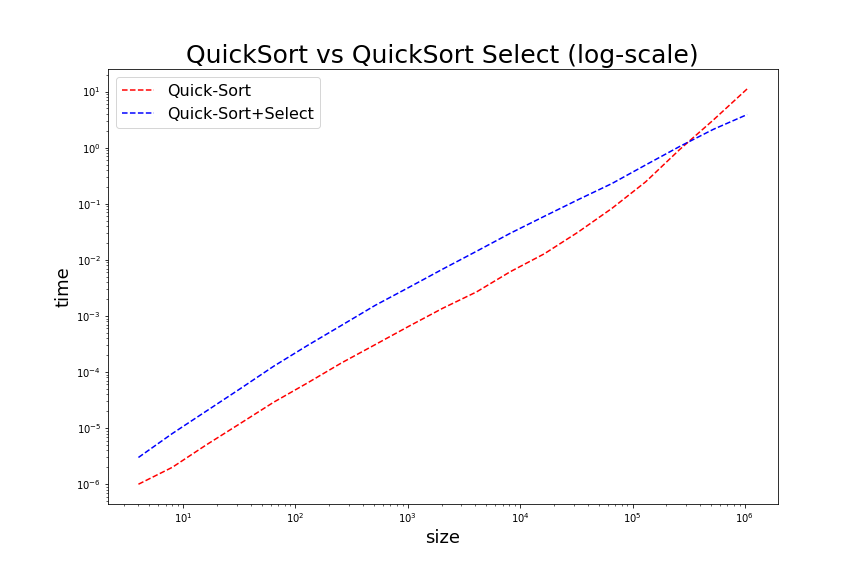
\includegraphics[width=1.1\textwidth]{../quicksort.png}  
		\caption{Benchmark of the \texttt{quick\_sort} method compared to its version when the \texttt{select} algorithm is involved in the selection of the pivot.}
		\label{plot}
	\end{figure}
	
	\noindent As it can be observed, the classic QUICK SORT has better performances on small list sizes. However, for big arrays the cost of partitioning becomes relevant and in those cases QUICK-SORT SELECT results to be more efficient.
	
\end{document}